\documentclass[a4paper,11pt]{report}
%\usepackage[none]{hyphenat}
%\usepackage[T1]{fontenc}
%\usepackage[bitstream-charter]{mathdesign}
%\usepackage[usenames,dvipsnames,pdf]{pstricks}
%\usepackage[crop=off]{auto-pst-pdf}
\usepackage{makeidx}
\usepackage{url}
\usepackage[square,sort,comma,numbers]{natbib}
\usepackage{framed}
\usepackage{makecell}
\usepackage{graphicx}
\usepackage{longtable}
\usepackage{amsfonts}
\usepackage{amsmath}
\usepackage[noend,ruled,noline,linesnumbered,algochapter]{algorithm2e}
\usepackage[linktoc=page]{hyperref}
\usepackage[margin=3cm]{geometry}
\usepackage{setspace} 
\usepackage{float}
\usepackage{fancyhdr}
\pagestyle{fancy}
\rhead{\nouppercase\leftmark}
\lhead{\nouppercase\rightmark}
\makeindex
\onehalfspacing 
\renewcommand*\contentsname{Table of Contents}
\begin{document}
\pagenumbering{roman}
%title page
\begin{titlepage}
\begin{center}

\vspace*{1cm}

{\LARGE \bf CREST: A Proactive Risk Mitigation \\[0.4em]
Framework for Symbolic Translation in\\[0.4em]
Neuro-Symbolic AI }

\vspace{0.5cm}
\line(1,0){380}

\end{center}
\vfill
\begin{center}
By
\end{center}
\vfill
\begin{center}
\begin{tabular}{lr}
\textbf{Md.\ Tanzamul Azad}   & \textbf{0112230863} \\[0.6em]
\textbf{Israt Jerin Porshi}   & \textbf{011221580}  \\[0.6em]
\textbf{Swarup Deb Nath}      & \textbf{0112230150} \\[0.6em]
\textbf{Jahidul Islam}        & \textbf{0112230654} \\[0.6em]
\textbf{Satyajit Kumar Baidya}& \textbf{011222168}  \\

\end{tabular}
\end{center}


\vfill
\begin{center}
{Submitted in partial fulfilment of the requirements \\of the degree of Bachelor of Science in Computer Science and Engineering}
\end{center}
\vfill
\begin{center}
{\today}
\end{center}
\vfill
	
\begin{center}

\includegraphics[scale=0.15]{./uiu}
\end{center}
\begin{center}
	\textsc{Department of Computer Science and Engineering\\
		United International University}
\end{center}
\end{titlepage}
\clearpage
\pagenumbering{roman}
\setcounter{page}{1}
%Abstract
\setlength{\headheight}{14pt}
\begin{center}
	{\huge \bf Abstract}
	\line(1,0){430}
\end{center}

  
\clearpage
\setlength{\headheight}{12pt}
\begin{center}
{\huge \bf Acknowledgements}
\line(1,0){430}
\end{center}






\clearpage
\setlength{\headheight}{14pt}
\begin{center}
{\huge \bf Publication List}
\line(1,0){430}
\end{center}

[Optional]


\section*{Journal Articles}
\begin{enumerate}
\item 
\end{enumerate}

\section*{Conference Papers}
\begin{enumerate}
\item 
\end{enumerate}


\section*{Additional Publications}

\begin{enumerate}
\item 
\end{enumerate}


  
\clearpage
\setlength{\headheight}{12pt}
\clearpage
\phantomsection
\tableofcontents
\renewcommand{\contentsname}{Table of Contents}
\addcontentsline{toc}{chapter}{Table of Contents}
\clearpage
\phantomsection
\addcontentsline{toc}{chapter}{List of Figures}
\listoffigures
\clearpage
\phantomsection
\addcontentsline{toc}{chapter}{List of Tables}
\listoftables
\clearpage
\pagenumbering{arabic}
\setcounter{page}{1}
\renewcommand\bibname{References}
\clearpage
\phantomsection
\chapter{Introduction}

In this chapter the project scope,motivation, objective, methodoly and expected results of the suggested CREST framework for proactive semantic risk detection and correction in Neuro-Symbolic AI pipelines are described.

\section{Project Overview}

At present, Neuro-Symbolic(Nesy) Artificial Intelligence has emerged as a leading example for building trustworthy and interpretable reasoning systems. Make a combination of the linguistic flexibility of Large Language Models(LLMs) with the formal correctness which is guaranteed by symbolic solvers. A populer design employs an LLM to convert natural alnguage statements into First Order Logic (FOL),which is subsequently sent to a symbolic theorem prover such as   Z3~\cite{demoura2008z3} for deductive inference. Although this design offers the best of both worlds,it hides a critical vulnerability at the translation boundary: the symbolic solver has no way to identify errors  when the LLM generates a syntactically valid but semantically flawed FOL formula .Without giving any warning,the solver returns an inaccurate conclusion after reasoning faithfully over an incorrect premise. We call these events as silent semantic failure,which impugns the very trustworthiness that Nesy systems were designed to provide.

In order to  fill this fundamental gap,this research presents \textbf{CREST} (\textbf{Corrective Risk Estimation for Symbolic Translation}), a proactive, training-free framework that intercepts LLM-generated FOL translations before they reach the symbolic solver. CREST determines the underlying error type, calculates a quantitative semantic risk score and directs high risk translations through a focused feedback driven correction loop. Combining deterministic predicate consistency checking, back translation semantic loss measurement and an LLM as judge diagnosis module, CREST serves as a semantic safety gate applicable to any off-the-shelf NeSy pipeline without requiring model retraining.

\section{Motivation}

NeSy systems are now being used more and more in critical fields where a single incorrect translation could have serious consequences. An omitted negation in a clinical statement such as patient has no history of penicillin allergy might be silently reversed in medical decision support. This can produce a wrong drug recommendation. In law, trying to follow the rules can actually turn into breaking them. If someone misunderstands a strict "pick only one" rule as a 'you can pick both' rule. A quantifier scope error causes a tight threshold requirement in financial regulation to change into a permissive rule. Through the same inference engine the symbolic solver receives both correct and incorrect translations to the symbolic solver in each domain,resulting in conclusions with identical apparent confidence and no cautions.2

The main problem of this vulnerability is the well established. Inaccuracy of LLM self-assessment for structured symbolic outputs. On FOL translation tasks,LLM often show overconfidence,generating high confidence results even when the underlying translation is completely wrong~\cite{savage2024do, yang2024harnessing}. Current correction techniques can be divided into two categories: reactive approaches that wait for the solver to produce error messages before attempting revision~\cite{pan2023logiclm}, and training-based techniques that require large enough expert annotated FOL corpora ~\cite{thatikonda2024strategies}. Sementtic translation risk is not estimated before solver execution. The main issue this research attempts to solve is developing such a proactive, training free safety system.

\section{Objectives}

The main goal of this research is to design,propose and empirically support a proactive,training free framework that intercepts and fixes semantically inaccurate LLM to FOL translations before they get to a symbolic solver. The following are the precise goal:

\begin{enumerate}
    \item To prove empirically that internal confidence signals cannot function as a safety gate in Neuro Symbolic pipelines and that LLM self reported confidence is an unreliable predictor of NL to FOL translations correctness.

    \item To determine and describe \textbf{cross-premise predicate naming inconsistency} as a quantifiable, predictable risk signal associated with translation instability in a variety of  multi-premise FOL reasoning tasks.

    \item To empirically show that when given semantically wrong but syntactically valid FOL,symbolic solvers like Z3 display slient semantic failure,leading to incorrect conclusions without issuing an error or warning.  

    \item To creat the \textbf{CREST framework}, a multi-component proactive pipeline that uses LLM as judge error diagnosis,deteministic predicate consistency checking, and back translation semantic loss measurement to assess translation risk prior to solver execution.

    \item To develop a \textbf{feedback-driven corrective re-translation mechanism} that allows the forward translator to fix high risk translations before symbolic inference by converting diagnostic outputs into targeted prompts.
\end{enumerate}

\section{Methodology}

The methodology of this project is organized into three coordinated layers :

\begin{enumerate}
    \item \textbf{Empirical Gap Characterization:} Three failure modes are identified  through a series of pilot experiments on the FOLIO benchmark~\cite{han2024folio} the quiet failure of Z3 on semantically incorrect FOL,the large cross premise predicate name inconsistency and the unreliability of LLM confidence on NL to FOL translation and the quiet failure of Z3 on semantically wrong FOL.The empirical foundation for the suggested framework is established by these experiments.

    \item \textbf{Proactive Risk Estimation Layer:} To remove same direction bias , a back translation module utilize a various model than the forward translator in order to translate generated FOL back into natural language.BERTScore is used to compare the back translated text with the original human written input~\cite{zhang2020bertscore},capturing the meaning level changes that surface measures such as BLEU and ROUGE systematically overlook.Targeting the particular cross premise failure mode found in earlier research, a parallel deterministic  predicate consistency checker finds predicate names that are lexically inconsistent but semantically equivalent across all premises of a tale. ~\cite{thatikonda2024strategies}.

    \item \textbf{Diagnostic and Corrective Layer:} When translations exceed the risk threshold, an LLM as a judge component receives them and produces a structured error diagnosis that details the type,severity and location of the issue within the FOL . Based on this diagnosis,the forward translator receives a personalized feedback prompt for retranslation. Translations below the threshold proceed directly to the Z3 solver ,avoiding the corrective layer.
\end{enumerate}

\section{Project Outcome}

The anticipated outcome of the research is complete, training-free framework for proactive semantic risk detection and correction at the LLM-to-symbolic translation boundary. This is supported by pilot experiments that motivate each design decision. Because CREST is domain-independent and solver agnostic , it can be deployed over any NeSy pipeline that changes natural language into formal symbolic representation prior to interfacae. Ultimately the finished product proves a fundamental proof of concept for a novel family of training free semantic safety methods that supplement current reactive correction techniques rather than taking their place.

\section{Organization of the Report}

The rest of this report is structured as follows.In \textbf{Chapter 2}  the state of the art  in NL to FOL translation, NeSy reasoning, uncertainty quantification and self-refinement for symbolic outputs is surveyed, and the gaps motivating CREST are identified.In  \textbf{Chapter 3}  the proposed CREST architecture is described.In \textbf{Chapter 4}  the pilot experiments are presented. Engineering standards, design constraints, and cost analysis are discussed in \textbf{Chapter 5} .Contribution is summarised, acknowledgment of pilot-stage limitations, and future assessment objective are outlined in \textbf{Chapter 6} 
\chapter{Background}

This chapter provides the foundational concepts needed to understand the remaining part of the report, provides a comprehensive literature review of related research and similar applications in the NeSy AI and NL to FOL translation literature, and develops the gap analysis motivating the proposed CREST framework.

\section{Preliminaries}

\textbf{Neuro-Symbolic (NeSy) AI} refers to architectures that combine sub-symbolic neural reasoning with symbolic logical inference. The neural component manages flexible natural language understanding, while the symbolic component enforces formal correctness over structured representations~\cite{colelough2025nesyreview}.

\textbf{First-Order Logic (FOL)} is a formal language for representing statements with quantifiers, predicates, and logical connectives, providing an exact, machine-verifiable representation of natural language meaning. Standard FOL builds include universal quantification ($\forall$), existential quantification ($\exists$), negation ($\neg$), conjunction ($\wedge$), disjunction ($\vee$), and implication ($\rightarrow$).

\textbf{Large Language Models (LLMs)} are deep neural networks trained on large text bodies capable of complex natural language understanding and generation. Within NeSy pipelines, LLMs serve as semantic parsers translating natural language premises into FOL, but prior work has consistently shown they make systematic errors when generating structured symbolic outputs~\cite{yang2024harnessing, thatikonda2024strategies}.

\textbf{NL to FOL Translation} is the task of converting natural language statements into corresponding FOL formulas, representing the critical interface between the neural and symbolic components of any NeSy reasoning pipeline. Errors can be syntactic, violating FOL grammar, or semantic, where the formula is grammatically valid but fails to keep the meaning of the original statement.

\textbf{Symbolic Theorem Provers} are deterministic systems that perform formal logical inference over symbolic representations. Z3~\cite{demoura2008z3}, a Satisfiability Modulo Theories (SMT) solver from Microsoft Research is the standard symbolic engine in modern NeSy pipelines. Z3 verifies logical consequences only with respect to its input formulas and has no mechanism for assessing whether those formulas correctly capture the intended meaning of the original natural language premises.

\textbf{Uncertainty Quantification (UQ)} refers to techniques for estimating model confidence in its predictions. In structured generation settings such as FOL translation, standard UQ methods become less reliable because the output space is combinatorial and semantically structured rather than smoothly distributed.

\textbf{BERTScore} is an approach that is  used to compare two sentences and determine how similar their meanings are. ~\cite{zhang2020bertscore}. Unlike n-gram-based metrics such as BLEU and ROUGE, BERTScore captures meaning-level changes including the loss of critical operators such as negation, making it well-suited for back-translation comparison scenarios.

\textbf{Back-Translation Consistency} is a technique where the system translates the output back into the source representation and comparing it against the original input. In the NL to FOL context, this produces a natural language paraphrase of the generated FOL that can be compared against the original human-written premise to estimate semantic preservation.

\textbf{LLM-as-Judge} refers to the use of a large language model as an evaluator that examines errors or assesses the quality of outputs produced by another model. This paradigm has emerged as a flexible alternative to rule-based classifiers for detecting nuanced or previously unobserved error types in structured generation tasks.

\textbf{The FOLIO Dataset} is a human annotated benchmark for FOL reasoning in natural language, consisting of 1,430 expert-written examples paired with ground-truth FOL annotations~\cite{han2024folio}. FOLIO's combination of natural language richness, multi-premise structure, and gold-standard FOL annotations makes it the standard benchmark for evaluating NL to FOL translation correctness and cross-premise consistency.

\section{Literature Review}

\subsection{Similar Applications}

Several systems and frameworks have been developed with objectives related to integrating natural language understanding with formal symbolic reasoning in NeSy pipelines.

\textbf{Logic-LM}~\cite{pan2023logiclm} is one of the most influential frameworks combining LLMs with symbolic solvers. The system translates natural language problems into symbolic formulations and delegates inference to deterministic solvers such as Z3 and Prover9, achieving substantial improvements over chain-of-thought prompting across five reasoning benchmarks. It introduces a self refinement module that uses solver error messages to revise incorrect formalizations. 

\textbf{LINC}~\cite{olausson2023linc} combines language models with FOL theorem provers for natural language inference. The system translates premises and hypotheses into FOL and uses an external prover for entailment, reporting complementary failure modes between purely neural and neuro-symbolic approaches. No mechanism is provided to estimate semantic risk before prover invocation.

\textbf{LogicLLaMA and MALLS}~\cite{yang2024harnessing} address NL to FOL translation through supervised fine-tuning of LLaMA-7B and LLaMA-13B on 28,000 GPT-4-generated NL-FOL pairs. While demonstrating GPT-4-level performance at reduced computational cost, the approach requires extensive training data, operates at the single-statement level, and does not address cross-premise consistency errors that arise in multi-premise reasoning.

\textbf{Strategies for Improving NL to FOL Translation}~\cite{thatikonda2024strategies} introduce ProofFOL and propose a multi-stage filtering pipeline with format correction, syntax validation, and semantic filtering. The authors fine-tune smaller models and explicitly acknowledge that realistic logical reasoning requires consistency of NL to FOL translations in predicate naming and logical operator usage across statements. However, their verifier requires fine-tuning on perturbation data, making it inapplicable as a training-free inference-time safety layer over arbitrary NeSy pipelines.

\textbf{SelfCheckGPT}~\cite{manakul2023selfcheck} demonstrates that consistency across multiple sampled outputs can serve as a hallucination detection signal for open ended language generation, using BERTScore, n-gram overlap, and natural language inference to assign hallucination scores. While the consistency principle is general, the evaluation focuses entirely on unstructured text. Direct transfer to structured FOL generation, where the output space is governed by formal semantics, stays underexplored.

Unlike the systems above, CREST integrates back-translation semantic loss measurement, deterministic predicate consistency checking, and LLM-as-Judge error diagnosis into a unified proactive pipeline operating before the symbolic solver executes and requiring no fine tuning of any model component. This combination addresses the core limitation left unresolved by all existing systems.

\subsection{Related Research}

Recent advancements across NeSy AI, NL to FOL translation, and consistency based uncertainty quantification collectively appreciate the present work.

Colelough and Regli~\cite{colelough2025nesyreview} conducted a PRISMA based systematic review of 167 NeSy papers from 2020 to 2024, finding that meta-cognition, the capacity of an AI system to monitor and adjust its own reasoning , appears in only five percent of reviewed papers. This finding directly motivates mechanisms that detect and correct translation errors before they actually propagate into symbolic inference.

A central line of work has focused on the quality and reliability of the NL to FOL translation step. Yang et al.~\cite{yang2024harnessing} demonstrated that even the most capable LLMs make systematic errors when translating single natural language statements into FOL. Thatikonda et al.~\cite{thatikonda2024strategies} expanded this to multi-premise scenarios, observing that cross-premise consistency in predicate naming and logical operator usage is both necessary for correct reasoning and consistently violated. Their work is the closest to ours in identifying predicate inconsistency as a critical failure mode but the proposed solution is training-based rather than proactive at inference time. Pan et al.~\cite{pan2023logiclm} and Olausson et al.~\cite{olausson2023linc} both demonstrated that reactive correction triggered by solver failure is insufficient, since syntactically valid but semantically wrong FOL passes their verification mechanisms undetected.

On the uncertainty quantification side, Savage et al.~\cite{savage2024do} found that LLMs frequently exhibit overconfidence in clinical decision tasks, producing high-certainty outputs even when the judgment is ambiguous,  a calibration failure that generalizes directly to the NL-to-FOL translation boundary. Manakul et al.~\cite{manakul2023selfcheck} showed that consistency-based sampling can detect hallucinations in open ended text, but applying this principle to structured FOL outputs requires care, since two semantically distinct FOL formulas may exhibit high token level similarity while two logically equivalent formulas may appear lexically different.

For measuring semantic preservation, BERTScore~\cite{zhang2020bertscore} has become a widely taken metric, leveraging contextual embeddings to capture meaning level differences that n-gram metrics miss. The FOLIO benchmark~\cite{han2024folio}, with its expert-annotated multi-premise stories and mechanically verifiable ground truth FOL annotations, provides the most suitable evaluation platform for studying both translation correctness and cross premise consistency.

Despite these collective advancements, no existing framework combines proactive risk estimation, deterministic cross premise consistency checking, and training free LLM-based error diagnosis into a unified pipeline that intercepts semantically incorrect FOL before symbolic inference. This is the specific gap CREST is designed to fill.

\section{Gap Analysis}

Recent advancements in NL to FOL translation, neuro-symbolic reasoning, and consistency based uncertainty quantification have demonstrated meaningful progress across individual components. However, several critical gaps persist that significantly limit their applicability to safe, training free deployment in real world Neuro-Symbolic pipelines:

\begin{itemize}

    \item Existing error correction strategies in NeSy pipelines are  \textbf{reactive}, relying on the symbolic solver to return error messages that subsequently trigger LLM based revision. This means that semantically incorrect but syntactically valid FOL passes through the verification mechanism undetected, since the solver verifies logical entailment over its input rather than the semantic faithfulness of the input to the original natural language.

    \item LLM self reported confidence has been shown to be \textbf{anti correlated with translation safety} in structured generation tasks, with high confidence outputs often being wrong. No existing NeSy pipeline incorporates an external risk estimation mechanism that operates independently of the LLM's own confidence signals at the translation boundary.

    \item \textbf{Cross premise predicate naming inconsistency} has been acknowledged in the literature as a critical semantic failure mode in multi premise NL to FOL translation, but existing solutions require supervised fine tuning on annotated FOL datasets. There is an absence of training free mechanisms that can detect predicate drift across premises at inference time.

    \item Consistency based hallucination detection methods such as SelfCheckGPT have been developed for \textbf{open ended natural language generation}, but their direct application to structured FOL generation is non trivial. Two semantically distinct FOL formulas may exhibit high token level similarity, and two semantically equivalent FOL formulas may exhibit low token level similarity, undermining naive consistency based risk signals.

    \item Most surface level similarity metrics such as BLEU and ROUGE are \textbf{insensitive to meaning level changes} such as the loss of negation or the inversion of quantifier scope. These metrics are therefore inadequate for measuring semantic preservation in back translation based risk estimation scenarios, where the most critical error modes involve single token operator changes that completely invert the meaning of a premise.

    \item Existing self refinement frameworks for symbolic translation generate corrective prompts based on \textbf{generic solver error messages} rather than on structured semantic diagnostics. As a result, the corrective signal lacks specificity about the type, location, and severity of the underlying translation error, limiting the effectiveness of re-translation.

    \item Symbolic theorem provers such as Z3 are \textbf{semantically blind} to the natural language origins of their input. When presented with a syntactically valid but semantically incorrect FOL formula; the solver returns a logically correct conclusion with respect to its input, producing an incorrect downstream answer with no error or warning. This phenomenon of silent semantic failure constitutes a fundamental safety vulnerability in any NeSy pipeline.

\end{itemize}
\begin{table}[h]
\centering
\label{tab:litreview}
\resizebox{\textwidth}{!}{%
\begin{tabular}{|p{3.5cm}|p{3cm}|p{3cm}|p{3cm}|p{4.5cm}|}
\hline
\textbf{ Reference}& \textbf{Problem Addressed} & \textbf{Methodology} & \textbf{Tools \& Datasets} & \textbf{Identified Gaps} \\
\hline
~\cite{colelough2025nesyreview}& Mapping of NeSy research landscape & PRISMA-based systematic review of 167 papers across five research areas & 2020-2024 NeSy literature corpus& Meta cognition is the least explored area at five percent of papers; self-monitoring at translation boundary is essentially absent\\
\hline
~\cite{pan2023logiclm}& LLM-symbolic integration for faithful reasoning & LLM to FOL translation followed by symbolic solver inference with self-refinement loop& ProofWriter, PrOntoQA, FOLIO, LogicalDeduction, AR-LSAT & Self refinement is reactive and triggered only by solver errors; semantically wrong but solver valid FOL bypasses the loop\\
\hline
~\cite{olausson2023linc}& Neurosymbolic NL inference using LLMs and FOL provers & Translation of premises and hypotheses to FOL with external prover based entailment checking& FOLIO and ProofWriter & No proactive semantic risk assessment before prover invocation; consistency across translations is not measured \\
\hline
~\cite{yang2024harnessing}& Improving NL-to-FOL translation via fine-tuning & Fine-tuning LLaMA-7B/13B on GPT-4 generated synthetic NL-FOL pairs with LoRA& MALLS (28k pairs) & Sentence level focus; multi-premise consistency not addressed; requires significant training resources and annotated data\\
\hline
~\cite{thatikonda2024strategies}& Translation error reduction via fine-tuning and verification & Incremental fine-tuning with predicate and FOL verifiers; categorization of syntactic and semantic errors & ProofFOL, FOLIO, ProofWriter & Verifier requires fine tuning on perturbation data; not directly applicable as a training free safety layer over arbitrary NeSy pipelines\\
\hline
~\cite{manakul2023selfcheck}& Consistency-based hallucination detection in LLMs & Sampling based comparison using BERTScore, n-gram, and QA-based variants& WikiBio passages from GPT-3 & Designed for unstructured open-ended text; direct transfer to structured FOL outputs is non-trivial due to surface-vs-semantic mismatch \\
\hline
~\cite{savage2024do}& Reliability and calibration of LLM outputs & Systematic evaluation of LLM confidence calibration across clinical scenarios & Clinical decision benchmarks & Confirms LLM self-confidence is unreliable for safety-critical tasks; no proposed external risk signal for structured translation \\
\hline
~\cite{han2024folio}& Evaluation of NL-FOL reasoning and translation & Expert-annotated multi-premise stories with ground-truth FOL formulas verified by FOL engine & FOLIO (1,430 examples) & A benchmark rather than a detection or correction method; reveals translation errors but provides no mechanism for proactive intervention \\
\hline
~\cite{zhang2020bertscore}& Semantic-aware evaluation of generated text & Contextual embedding-based token similarity with precision, recall, and F1 & 363 MT and image captioning systems & A general purpose metric not applied to NeSy translation risk; known insensitivity to quantifier scope changes requires complementary signals\\
\hline
~\cite{demoura2008z3}& Formal symbolic inference & Satisfiability Modulo Theories solver for FOL with multiple background theories & Software verification benchmarks and academic NeSy pipelines & Verifies entailment over input formulas only; cannot detect that input FOL is semantically inconsistent with original NL premise\\
\hline
\end{tabular}%
}
\caption{Literature Review Summary with Identified Gaps}
\end{table}

\section{Summary}

Research on translating natural language into formal logic, neurosymbolic reasoning, and using consistency to measure uncertainty has come a long way. We've seen real progress through end-to-end frameworks, models fine-tuned to catch errors, and sampling-based methods for spotting hallucinations. That said, there's still plenty left to figure out. Existing self refinement systems operate reactively after solver failure rather than proactively before execution. Fine-tuning based verifiers cannot serve as inference time safety layers over arbitrary pre existing pipelines. Consistency based detection methods have been validated on unstructured natural language, not structured symbolic outputs where the surface vs. semantic relationship is qualitatively different. Surface level metrics fail to detect critical meaning level changes such as negation loss and quantifier scope inversion. Crucially, no existing solution integrates back translation semantic loss measurement, deterministic predicate consistency checking, and structured LLM based error diagnosis into a coherent training free framework that intercepts semantically incorrect FOL before it reaches the symbolic solver. The proposed CREST framework directly addresses these crucial gaps.
\chapter{Project Design}

It describes the core analysis of the requirements and the outline of the functional and non-functional aspects of the proposed CREST framework needed for proactive semantic risk detection in Neuro-Symbolic AI pipelines. Here are also the data flow diagrams at several levels. They describe the methodology and architectural components, while designing it justifies about the other solutions. Also discusses why it is taken or why which one is not. Lastly, discussed the task management of the team.  

\section{Requirement Analysis}

The most needed requirements are initially API of LLMs for forward translation and for back translation we initially decided to use another LLM, later there will be used a self made verbalizer. Also need predicate checker which runs by CPU and symbolic solver. The BERTScore package~\cite{zhang2020bertscore}, and the Z3 SMT solver bindings~\cite{demoura2008z3} are one of the core requirements here.

\subsection{Functional Requirements}

\begin{enumerate}
    \item \textbf{Forward FOL Translation:} The framework use a Large Language Model to translate each natural language premise into a First-Order Logic formula maintaining solver-compatible syntax.
    
    \item \textbf{Back-Translation and Semantic Loss Estimation:} The system does reverse translation of each generated FOL into natural language using a model distinct from the forward translator, then shows a risk score by computing semantic similarity between the back-translated text and the original premise.

    \item \textbf{Cross-Premise Predicate Consistency Checking:} The framework applies deterministic regex extraction and edit-distance comparison across all FOL formulas of a story to identify semantically similar but lexically inconsistent predicate names~\cite{thatikonda2024strategies}.

    \item \textbf{Risk-Based Routing:} The system combines two scores, one is coming from semantic loss (BERTScore) and another is from predicate risk and decide whether it should proceed to solver or not.

    \item \textbf{Error Diagnosis:} For premises scored high, the framework directs it to an LLM-as-Judge component~\cite{zheng2023judging} that returns a structured diagnosis having error type, severity, location, and feedback.

    \item \textbf{Feedback-Driven Re-translation:} The system converts the diagnosis into a feedback prompt and sends back it to the forward translator. It translates again and iterates the whole process again to pass the risk threshold.
\end{enumerate}

\subsection{Non-Functional Requirements}

\begin{enumerate}
    \item \textbf{Training-Free Operation:}  The Framework fully works at inference time, and no model fine-tuning is required. Thus, it can be directly used with any off-the-shelf Neuro-Symbolic pipeline, and the extra data and compute needed for supervised training can be ignored. 

    \item \textbf{Reproducibility:} The pipeline is designed in a way that, in every iteration of execution, we get the same result. That’s why fixed random seeds are used; intermediate output is logged in a structured way and LLM endpoint and Python dependencies exact versions are pinned there. 

    \item \textbf{Modularity:} Each part of the pipeline follows the same contract or guideline for the same input and output. As a result, the forward translator, back translator, similarity metric, predicate checker, or judge all the components can be replaced or changed individually, without changing the whole system. 

    \item \textbf{Cost Efficiency:} The Routing Mechanism is designed in a way that expensive LLMs as a judge or retranslation can only be used in high-risk or flagged cases. Thus, in the case of safe inputs, it results in less cost and latency. 
    \item  \textbf{Solver Agnosticism:} Though Z3 is used in the current implementation, this framework doesn’t rely on any specific symbolic server. By making a small change in the interface, it can be used with other FOL or SMT solvers. 
\end{enumerate}

\subsection{Data Flow Diagram}

The data flow within the CREST framework is represented across three levels of diagram. Figure~\ref{fig:dfd0} presents the Level 0 context diagram, Figure~\ref{fig:dfd1} expands the internal process structure, and Figure~\ref{fig:dfd2} details the component-level data exchange.

\begin{figure}[H]
\centering
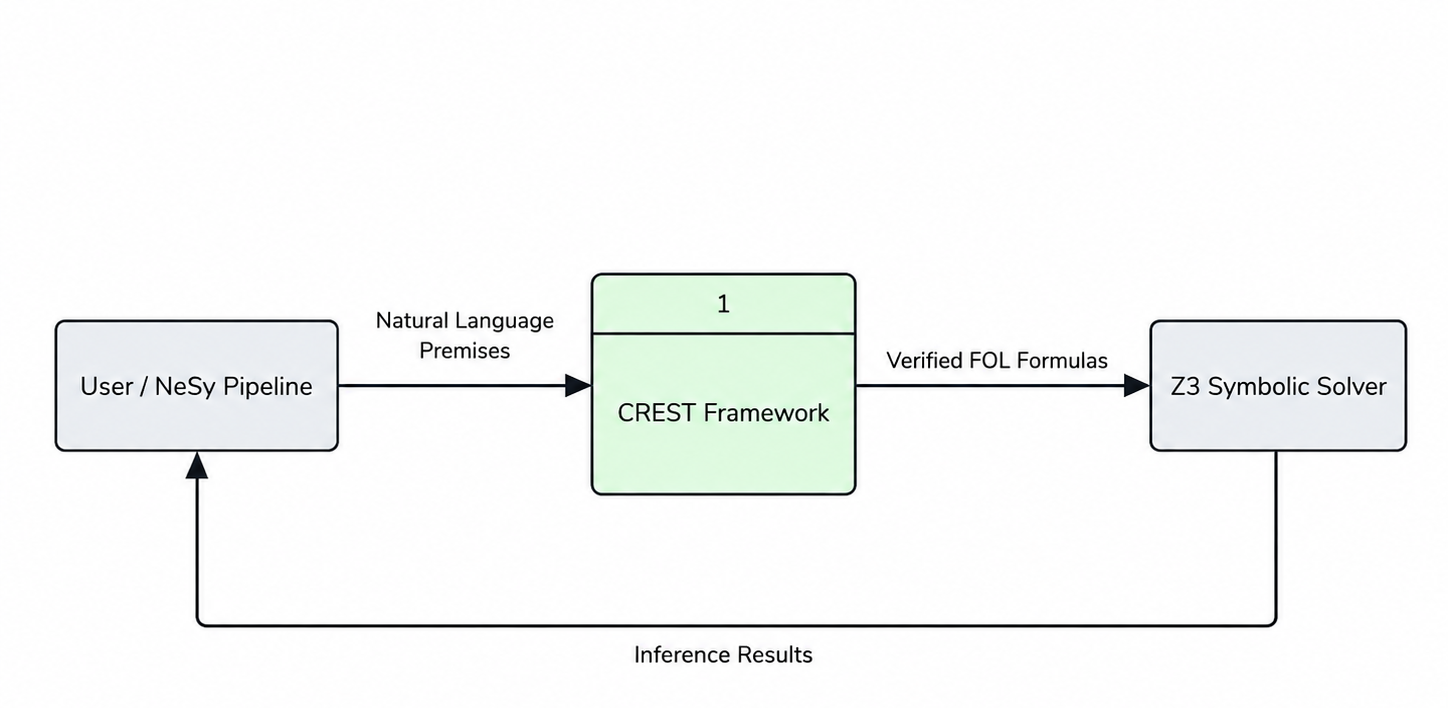
\includegraphics[width=0.85\textwidth]{./figures/dfd1.png}
\caption{DFD Level 0}
\label{fig:dfd0}
\end{figure}

\begin{figure}[H]
\centering
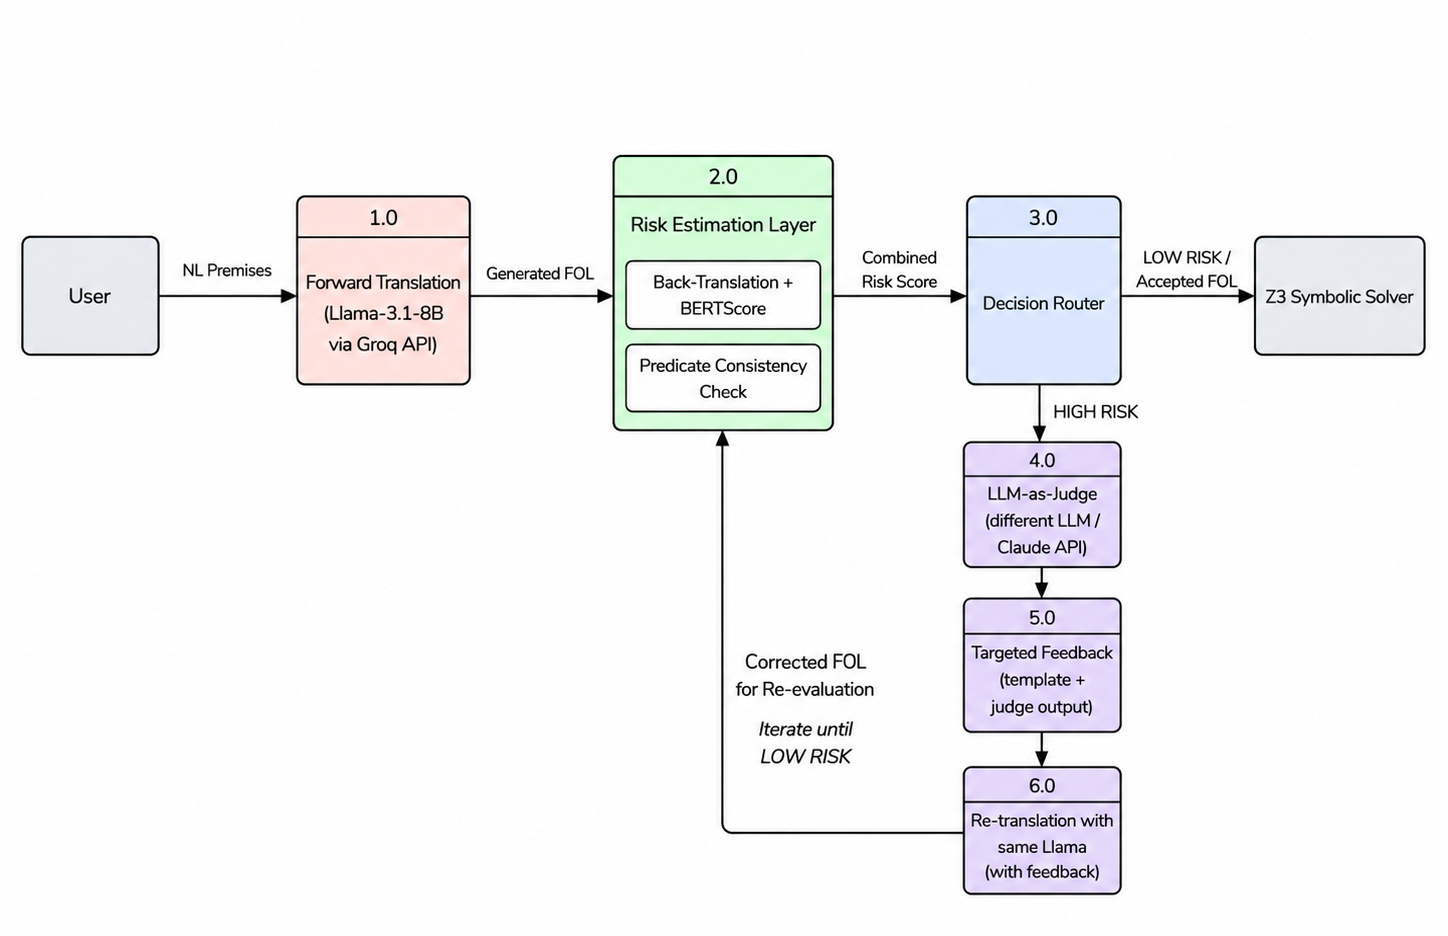
\includegraphics[width=0.95\textwidth]{./figures/dfd2.png}
\caption{DFD Level 1}
\label{fig:dfd1}
\end{figure}

\begin{figure}[H]
\centering
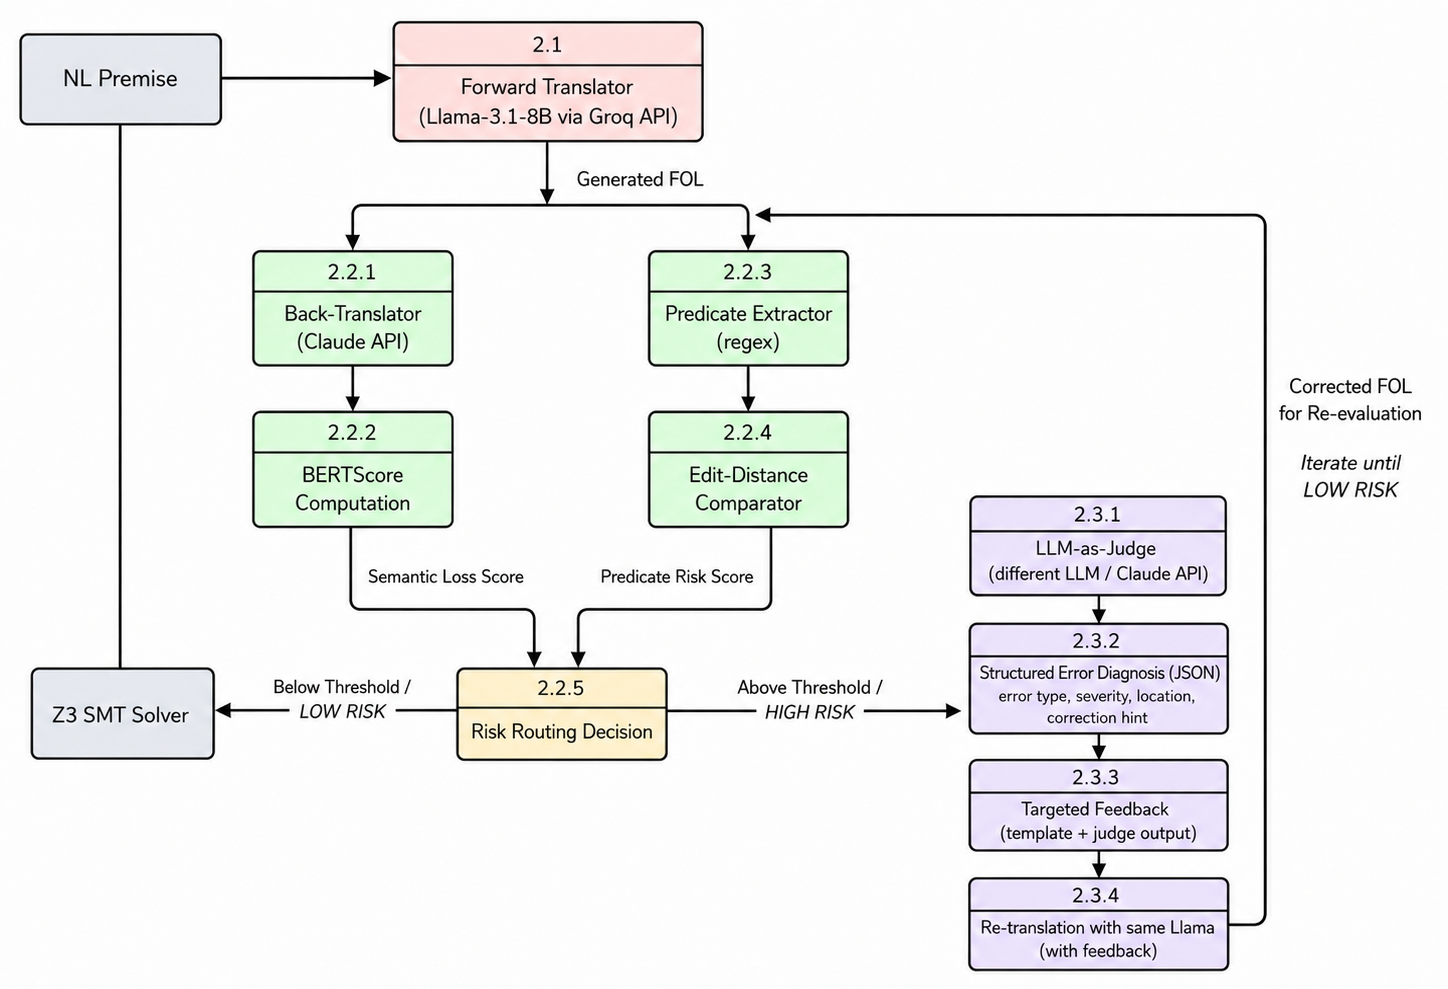
\includegraphics[width=\textwidth]{./figures/dfd3.png}
\caption{DFD Level 2}
\label{fig:dfd2}
\end{figure}

\section{Detailed Methodology and Design}

The CREST framework try to find out the fundamental safety gap at the translation limitation of Neuro-Symbolic AI pipelines. Large Language Models produce FOL translations that are syntactically valid but semantically incorrect, and symbolic theorem provers downstream have no mechanism to detect this category of error. AI logic tools do exactly what they are told. If you give them bad information, they will give you an answer that seems perfectly logical but is actually completely wrong. We call this a hidden mistake. Current fixes usually only kick in when the computer shows an error message. But this means they completely miss the bad information that the computer accepts without complaining. formulas~\cite{pan2023logiclm}, and supervised fine-tuning of dedicated verifiers, which requires annotated data~\cite{thatikonda2024strategies, yang2024harnessing}. our pipeline addresses this gap by cut off LLM-generated FOL before symbolic inference, estimating a quantitative risk score from complementary signals, diagnosing the underlying error type, and routing flagged translations through a feedback-driven correction loop. The overall architecture is depicted in Figure~\ref{fig:architecture}.

\begin{figure}[H]
\centering
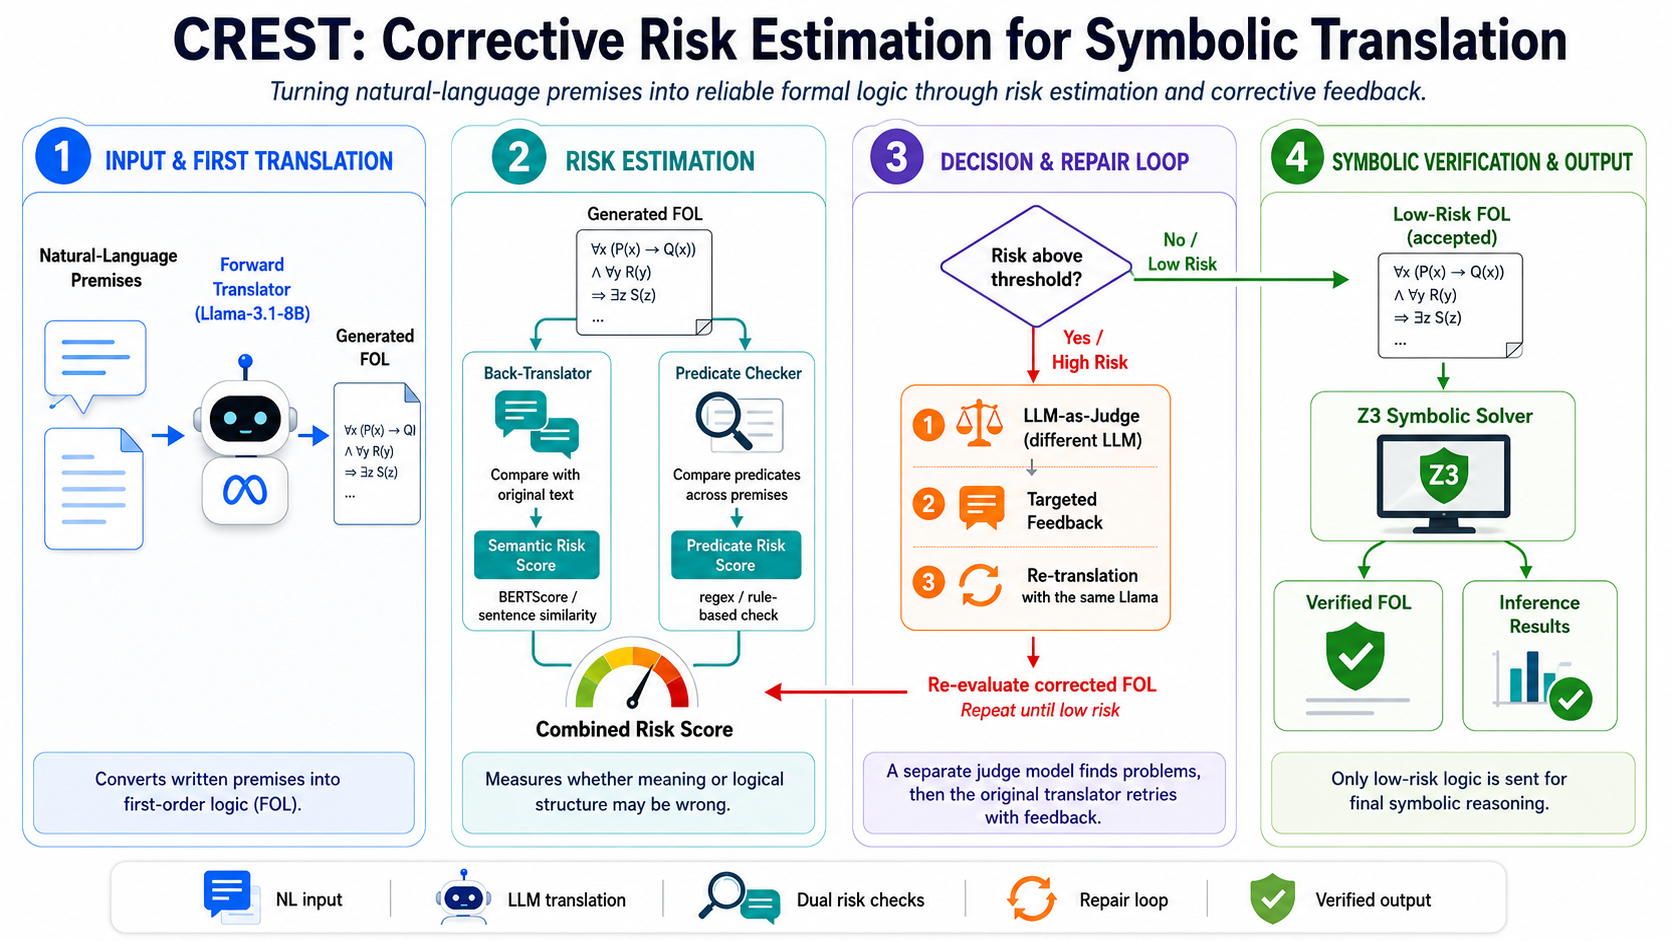
\includegraphics[width=\textwidth]{./figures/CREST.png}
\caption{Entire Architecture of the CREST Framework}
\label{fig:architecture}
\end{figure}

\subsection{Dataset}

The FOLIO benchmark~\cite{han2024folio} is used for evaluation. FOLIO is an expert-annotated dataset of 1,430 examples spanning 487 premise sets, paired with gold-standard FOL annotations that are mechanically verifiable by an FOL inference engine. We selected FOLIO because it provides ground-truth FOL at the story level rather than the isolated sentence level, enabling the cross-premise consistency analysis that constitutes a core component of the framework, and because its premises are written by human experts rather than generated from synthetic templates. For FYDP 1, a subset of 45 manually annotated premises and 20 multi-premise stories was used.In FYDP 2 will extend evaluation to the full benchmark and to ProofWriter for generalization testing.

\subsection{Forward Translation Module}

The forward translation module consumes a natural language premise and produces a corresponding FOL formula which is compatible with the Z3 solver. The module uses Llama-3.1-8B accessed through the Groq API, to balance between translation quality and inference cost. The Groq free academic tier provides sufficient token for full-scale evaluation across FOLIO. A fixed temperature of 0.1 balances deterministic behaviour with the controlled required for sampling-based analysis.

\subsection{Back-Translation and Semantic Loss Module}

The back-translation module receives the generated FOL and converts it back into natural language using the Anthropic Claude API. Using a separate model for back-translation is well-thought if the same LLM performed both directions, a systematic error such as a dropped negation could be silently reproduced in the backward direction, masking the error from comparison. The back-translated NL is compared against the original premise using BERTScore~\cite{zhang2020bertscore}, which detect meaning-level changes such as negation loss that n-gram metrics like BLEU and ROUGE systematically miss. The semantic loss signal is computed as
\[
\text{loss}_{\text{sem}} = 1 - \text{BERTScore}(\text{NL}_{\text{orig}}, \text{NL}_{\text{back}}).
\]

\subsection{Predicate Consistency Module}

The predicate consistency module operates in parallel with back-translation and analyzes the full set of FOL formulas for a story without any LLM . The module extracts predicate names from the FOL using regex-based parsing, then computes pairwise edit-distance similarity. Predicate pairs whose normalized similarity falls in the range $(0.6, 1.0)$ are flagged as suspicious, till pairs in this range typically represent the same concept expressed with minor difference such as \texttt{GoToBuilding} and \texttt{GoesToBuilding}. The module produces a binary risk flag and a quantitative predicate risk score equal to the fraction of predicates involved in suspicious pairs. The design ensures full reuse and zero API cost, complementing the neural back-translation signal.

\subsection{Risk Routing Module}

The risk routing module join the two signals and make them into a routing decision. A premise enters the corrective loop if either the semantic loss  surpass $\theta_{\text{sem}}$ or the predicate risk score exceeds $\theta_{\text{pred}}$:
\[
\text{Route to corrective loop} \iff (\text{loss}_{\text{sem}} > \theta_{\text{sem}}) \lor (\text{risk}_{\text{pred}} > \theta_{\text{pred}}).
\]
The premises that fail not either condition bypass the corrective loop and proceed directly to the symbolic solver. For balancing memory and precision on the error detection task, the thresholds are measured against the manually annotated pilot subset.

\subsection{LLM-as-Judge Module}

After receiving flagged premises along with their authentic NL,generated FOL ,back translated NL and risk score the LLM as judge module gives a structured JSON diagnostic ~\cite{zheng2023judging}. The Anthropic Claude API is used to implement the module. The judge returns four fields: error type drawn from \texttt{NEGATION\ LOSS}, \texttt{QUANTIFIER\ ERROR}, \texttt{XOR\ COLLAPSE} or \texttt{OTHER} severity rated as \texttt{CRITICAL}, \texttt{HIGH}, \texttt{MEDIUM} or \texttt{LOW}. The location of the inconsistency in the FOL and a suggestion for correction are included. The LLM judge is used instead of a rule based system because semantic errors can be unpredictable. The deterministic predicate checker covers only known errors, while the judge provides the flexibility needed to identify novel cases.

\subsection{Feedback-Driven Re-translation Module}

The re-translation module converts the judge's diagnosis into a feedback prompt using deterministic templates indexed by error type. The prompt explicitly identifies the error type and points to the affected component of the FOL, instructing the forward translator to produce a corrected version with attention to the diagnosed issue. The forward translator is re-invoked with this feedback-augmented prompt, producing a corrected FOL that is then passed to Z3. Unlike reactive self-refinement loops that operate on generic solver error messages~\cite{pan2023logiclm}, the CREST feedback mechanism uses structured semantic diagnostics, enabling targeted correction rather than generic retry.

\section{Alternative Solutions Considered}

There were other alternatives too, but those are removed because of some specific reason.
There can be used same model for back translation, but the decision is denied because, if the same model does the forward translation, it can be biased or do the same mistake silently while back translation too.
To identify semantic changes, we need some systematically sensitive metrics. That's why, surface level metric (BLEU, ROUGE) were not considered. 
Rule based error classifier was denied because, it is totally hard-coded and it can't able to find semantic differences.
Detecting consistency ~\cite{manakul2023selfcheck}  of results was also rejected because it doesn't flag error properly. Wrong results can be consistent without any feedback.

\section{Task Allocation}

The CREST framework is a hybrid model that integrates natural language processing, symbolic reasoning, semantic difference checking, and structured LLM-based evaluation. The team of five members did a deep research about this framework. Two members are allocated for the forward and back-translation pipeline, including API integration, prompt design, and request orchestration. One member is allocated for the deterministic predicate consistency module, including regex extraction, edit-distance computation, and threshold calibration. One member is allocated for the LLM-as-Judge module and feedback templates, including structured JSON prompt engineering and error taxonomy refinement. One member is responsible for the Z3 integration, the end-to-end evaluation pipeline, and the experimental analysis including manual annotation and statistical evaluation against ground truth. All team members contribute to the literature review, design discussions, and documentation, with regular  meetings to ensure consistent integration for the framework.

\section{Project Plan}

The CREST framework will be developed across two phases. In FYDP 1, three pilot experiments on the FOLIO benchmark to show the core gap, high-confidence LLM translations contain frequent semantic errors, cross premise predicate naming inconsistency is huge in LLM-generated FOL, and Z3 silently accepts semantically incorrect translations without any error signal. The deterministic Predicate Consistency Checker and Risk Scoring Framework have been partially implemented using regex-based predicate extraction and normalized edit distance, where LLM involvement is not required. In FYDP 2, the full pipeline will be deployed end-to-end across multiple benchmarks including FOLIO, ProofWriter, and PrOntoQA. The forward translator (Llama 3.1 8B) will run locally for generaing FOL, the back-translator will be replaced by a rule-based FOL-to-NL verbalizer, and the LLM-as-Judge component will be replaced by a lightweight risk-guided feedback fine tuned model which will be  trained by  using the combined risk score to make better re-translated FOL. The complete framework will be evaluated using precision, recall, and F1 on risk detection, alongside Z3 reasoning accuracy before and after CREST correction.

\section{Summary}

Chapter 3 explained how the CREST system is built, how it works, and who on the team is doing what. It started by listing exactly what the system needs to do to catch hidden errors early. We used clear diagrams to show step-by-step how data enters, moves through, and leaves the system. The chapter also broke down every single part of the tool like the translators, error checkers, and the AI judge that helps fix mistakes. We even explained why we rejected other design ideas. Finally, we listed the jobs for our five team members, giving us a clear plan to build and test everything in the next phase (FYDP 2).
\input{4.implementation.tex}
\chapter{Standards and Design Constraints}

This chapter outlines the engineering standards and professional codes of conduct for the proposed CREST framework, along with the design constraints, cost analysis, and complex engineering problem mapping relevant to the project.

\section{Compliance with the Standards}

Designing a framework that integrates Large Language Models, symbolic theorem provers, semantic similarity metrics, and structured LLM-based diagnosis requires adherence to established engineering standards. The following sections detail how CREST aligns with these professional guidelines.

\subsection{Software Standards}

\textbf{Fundamental Canons of ASME Code 2:}\\
Engineers will perform services only in areas of their competence. This project falls within Computer Science and Engineering, specifically Artificial Intelligence, Natural Language Processing, Formal Methods, and Symbolic Reasoning, all within the academic and professional competence of the development team.

\textbf{ACM Code of Professional Responsibilities Code 2.2:}\\
Maintain high standards of professional competence, conduct, and ethical practice. The framework adheres to rigorous professional standards, which is particularly important given that semantically incorrect FOL translations propagating through symbolic solvers can produce confidently wrong conclusions in any downstream application.

\textbf{ACM Code of Professional Responsibilities Code 2.3:}\\
Know and respect existing rules pertaining to professional work. Use of third-party LLM APIs (Groq, Anthropic) is conducted strictly within each provider's terms of service and rate-limit policies, and all evaluation datasets including FOLIO are accessed under their specified licenses.

\textbf{ACM Code of Professional Responsibilities Code 2.4:}\\
Give comprehensive and thorough evaluations of computer systems and their impacts. The team has explicitly documented component-level limitations: BERTScore's reduced sensitivity to quantifier-scope changes, the predicate checker's restriction to programmed lexical drift patterns, and the LLM-as-Judge's requirement for empirical validation against ground-truth annotations.

\textbf{ACM Code of Professional Responsibilities Code 2.5:}\\
Perform work only in areas of competence. The solution addresses a challenge within Computer Science and Engineering by combining natural language processing, formal logic, symbolic verification, and uncertainty quantification, all within the team's field of study.

\textbf{ACM Code of Professional Responsibilities Code 2.6:}\\
Access computing and communication resources only when authorized. All API access uses individually issued credentials, and no unauthorized data scraping or credential sharing is performed at any stage of the project.

\textbf{ACM Code of Professional Responsibilities Code 2.7:}\\
Design and implement systems that are robustly and usably secure. The framework incorporates deterministic checks (predicate consistency via regex and edit distance) alongside neural components (BERTScore and LLM-as-Judge), ensuring at least one risk signal remains available even if a neural component degrades.

\textbf{IEEE Code of Ethics Code 6:}\\
Maintain technical competence in software and hardware. The system design draws on the team's background in natural language processing, formal verification, and NeSy systems literature, supplemented by review of recent ACL, EMNLP, NeurIPS, and ICLR publications.

\subsection{Hardware Standards}

\textbf{Fundamental Canons of ASME Code 2:}\\
Engineers shall perform services only in areas of their competence. Managing the hardware requirements, including GPU-backed cloud inference for the forward translator and CPU-based execution for symbolic solving and deterministic checking, falls within the technical capabilities of the development team.

\textbf{ACM Professional Responsibilities Code 2.3:}\\
Know and respect existing rules pertaining to professional work. Cloud computing environments including Google Colab and Kaggle are accessed within the standard academic-tier usage limits of each platform.

\textbf{ACM Professional Responsibilities Code 2.4:}\\
Give comprehensive and thorough evaluations of computer systems and their impacts. Hardware failure risks such as transient API unavailability and rate-limit throttling are mitigated through retry logic, deterministic caching of intermediate outputs, and reproducible random seeds.

\textbf{ACM Professional Responsibilities Code 2.6:}\\
Design and implement systems that are robustly and usably secure. All intermediate pipeline outputs (forward FOL, back-translated NL, BERTScore values, judge diagnoses) are logged in structured form for independent verification and reproducibility.

\subsection{Communication Standards}

\textbf{ASM General Ethical Principles Code 1.3:}\\
Be honest and trustworthy. CREST produces risk scores explicitly accompanied by their underlying signals (semantic similarity score, predicate inconsistency rate, judge-diagnosed error type), allowing any downstream user to trace the source of a flagged translation rather than receiving an opaque number.

\textbf{IEEE Code of Ethics Code 4:}\\
Avoid unlawful conduct.
\begin{itemize}
    \item All datasets, including FOLIO, are used in accordance with their original licensing terms.
    \item No private, sensitive, or personally identifiable information is processed by the system. All evaluation inputs are drawn from public benchmarks.
    \item API integrations with Groq and Anthropic are conducted using authorized credentials and within published terms of service.
    \item Outputs of the system are clearly labeled as automated risk estimates and are not represented as authoritative judgments on the correctness of any particular FOL formula.
\end{itemize}

\subsection{Societal Standards}

\textbf{Fundamental Principles of ASME Code 1:}\\
Using knowledge and skills for the enhancement of human welfare. CREST directly addresses silent failure in AI systems that could produce confidently incorrect outputs in high-stakes domains, contributing to safer deployment of AI-driven reasoning systems.

\textbf{Fundamental Principles of ASME Code 4:}\\
Supporting the professional and technical societies of their disciplines. The literature review and citations acknowledge contributions across NL-to-FOL translation, NeSy AI, uncertainty quantification, and LLM-as-Judge research, strengthening the shared professional knowledge base.

\textbf{ACM General Ethical Principles Code 1.1:}\\
Contribute to society and to human well-being. By reducing the rate at which semantically incorrect symbolic translations reach downstream solvers, the framework supports more reliable AI-driven decision-making in any application dependent on formal reasoning over natural language inputs.

\textbf{ACM General Ethical Principles Code 1.4:}\\
Be fair and take action not to discriminate. The evaluation methodology tests the framework across the full diversity of premise types and reasoning patterns in the FOLIO benchmark, rather than restricting evaluation to cases where the framework is expected to perform well.

\textbf{ACM General Ethical Principles Code 1.6:}\\
Respect privacy. The framework processes only publicly available benchmark data and does not store, log, or transmit any user-provided sensitive inputs in its evaluation pipeline.

\textbf{ACM General Ethical Principles Code 1.7:}\\
Honor confidentiality. No confidential information is involved in the development or evaluation of the system. All datasets, code, and results are intended to be reproducible and publishable.

\textbf{ACM Professional Leadership Code 3.1:}\\
Ensure that the public good is the central concern during all professional computing work. Improving the safety of NeSy AI systems is a direct public-good concern as such systems are increasingly deployed in domains affecting human welfare.

\textbf{IEEE Code of Ethics Code 1:}\\
Ensure the safety of the public and the environment. The proactive risk-estimation layer in CREST is specifically designed to prevent silent semantic failure in symbolic reasoning pipelines, contributing to the safety of any downstream system relying on formal logical inference.

\textbf{IEEE Code of Ethics Code 7:}\\
Avoid discrimination. The framework operates on structural and semantic properties of FOL translations and does not consume demographic, identity-based, or otherwise sensitive features that could introduce discriminatory bias.

\section{Design Constraints}

\subsection{Economic Constraint}
The framework incurs computational costs primarily from LLM API calls for forward translation, back-translation, and LLM-as-Judge diagnosis. The forward translator uses Llama-3.1-8B via the Groq API free academic tier. The back-translator and judge use the Anthropic Claude API, a pay-per-token service. Budget constraints affect the scale of the full evaluation, and the routing mechanism minimizes cost by invoking the judge and re-translation loop only for high-risk translations rather than every input.

\subsection{Environmental Constraint}
Large language model inference contributes to a measurable carbon footprint at scale. CREST mitigates this through three design choices .The predicate consistency checker runs locally on the CPU with negligible energy cost. The routing mechanism restricts expensive neural diagnosis to high-risk inputs, and the use of Llama-3.1-8B rather than a frontier-scale model significantly reduces per-call energy consumption during the most frequent pipeline step.

\subsection{Ethical Constraint}
CREST processes only natural language and FOL representations of logical reasoning problems and does not consume sensitive user data. The framework produces risk scores, not correctness judgments. Downstream users must understand that a low risk score does not guarantee semantic correctness and that a high risk score does not constitute a definitive verdict of error. This positioning is intended to prevent over-depended on automated risk estimation in safety-critical settings.

\subsection{Social Constraint}
New safety layers adoption in AI pipelines often faces resistance from developers who view additional verification steps as latency or cost overhead. CREST's training-free design allows insertion into any existing NL-to-FOL pipeline without retraining the underlying models. The routing mechanism ensures the additional cost is incurred only for high-risk translations, preserving the latency profile on safe inputs and lowering the operational barrier to adoption.

\section{Cost Analysis}

The CREST framework operates within a resource-conscious academic budget. The primary paid components are the back-translation and diagnostic API calls via the Anthropic Claude API. The forward translator uses the Groq API free academic tier. All remaining components rely on open-source licensing and free compute environments. All costs are reported in Bangladeshi Taka (BDT).

\begin{table}[htbp]
\centering
\renewcommand{\arraystretch}{1.4}
\begin{tabular}{|p{2.8cm}|p{7.8cm}|r|}
\hline
\textbf{Component} & \textbf{Specification} & \textbf{Cost (BDT)} \\
\hline
Forward Translator API &
Llama-3.1-8B via Groq API free academic tier for NL-to-FOL forward translation. &
0 \\
\hline
Back-Translation API &
Anthropic Claude API for FOL-to-NL back-translation across approximately 1,430 FOLIO premises, plus retries and additional benchmark extensions. &
3,000 \\
\hline
LLM-as-Judge API &
Anthropic Claude API for structured error diagnosis. &
2,000 \\
\hline
Cloud GPU Compute &
Google Colab Pro subscription for full-scale BERTScore computation, embedding model experimentation, and Z3 batch execution. &
5,000 \\
\hline
On-Demand GPU Rental &
Occasional RunPod on-demand GPU access for stress testing, local Llama inference fallback, and ablation experiments outside Colab session limits. &
4,500 \\
\hline
Evaluation Datasets &
FOLIO~\cite{han2024folio} via Hugging Face open license. ProofWriter and additional benchmarks via their respective open releases. &
0 \\
\hline
Solver and Libraries &
Z3 SMT Solver~\cite{demoura2008z3}, BERTScore, Hugging Face Transformers, and supporting Python libraries under open-source licenses. &
0 \\
\hline
Contingency Buffer &
Reserve for API overage charges, additional sampling runs during ablation studies, and unexpected scaling needs. &
4,000 \\
\hline

\multicolumn{2}{|r|}{\textbf{Total Allocated Budget}} &
\textbf{BDT 18,500} \\
\hline
\end{tabular}
\caption{Project Cost Analysis  6-Month Development and Evaluation Lifecycle}
\label{tab:project_cost_analysis}
\end{table}

\noindent\textit{Zero-cost components rely on open-source licensing and free-tier API access, ensuring full reproducibility in resource-constrained research environments. The training-free design eliminates fine-tuning costs that dominate comparable NeSy research budgets.}
\clearpage

\section{Complex Engineering Problem}

\subsection{Complex Problem Solving}

A project constitutes a complex engineering problem if it satisfies any criteria from P1 to P7. The following maps the CREST framework against these Knowledge and Problem Profiles.

\textbf{P1: Depth of Knowledge Required.}
P1 is satisfied when one or more of K3 through K8 are fulfilled.

\textbf{K3: Engineering Fundamentals:} The framework employs edit-distance algorithms for predicate name comparison, regex-based FOL component extraction, and modular pipeline architecture for routing between components, directly applying data structures and string-matching fundamentals.

\textbf{K4: Specialist Knowledge:} Integration of Large Language Models, FOL translation, SMT solvers, contextual-embedding-based semantic similarity, and LLM-as-Judge diagnosis demonstrates specialist knowledge extending well beyond standard undergraduate curricula.

\textbf{K5: Engineering Design:} Standard library functions are insufficient. The framework requires custom design of a back-translation semantic loss signal, a deterministic cross-premise predicate consistency checker, an LLM-as-Judge prompt structure for FOL error diagnosis, and a feedback-template system converting structured diagnoses into targeted re-translation prompts.

\textbf{K6: Knowledge of Engineering Practice:} The project follows software engineering best practices including version control via Git, reproducible execution through Jupyter and Colab notebooks, modular API-based architecture, and structured logging of all pipeline outputs.

\textbf{K7: Contextual Awareness:} The framework is explicitly framed as a safety layer rather than a definitive verifier, with the team having considered the implications of deploying such a system in high-stakes domains where silent semantic failure can cause real harm.

\textbf{K8: Research Literature:} The extensive literature review draws from ACL, EMNLP, NeurIPS, ICLR, and TACAS, satisfying the requirement for engagement with current research literature.

Fulfilling K3 through K8 confirms that the project successfully meets the P1 requirement.

\textbf{P2: Range of Conflicting Requirements.}
The CREST system has to balance a few tough choices. Bigger AI models check work better, but they are slow and cost more. Being super strict catches more mistakes, but it also creates extra work by falsely flagging good translations. Also, the basic checker is very consistent, but only the smart AI can spot new, unusual errors. By testing and finding the perfect balance between all these things, the system meets the P2 requirement.

\textbf{P3: Depth of Analysis Required.}
No obvious solution exists for proactive, training-free NL-to-FOL safety. Existing approaches are either reactive (relying on solver feedback) or training-based (requiring annotated corpora). Designing a proactive inference-time safety layer required identifying risk signals and combining them with a structured diagnostic component, a non-trivial design problem satisfying P3.

\textbf{P4: Familiarity of Issues.}
Combining back-translation semantic loss, deterministic predicate alignment, and LLM-as-Judge diagnosis into a unified proactive pipeline for symbolic translation is a frontier research direction without standard textbook solutions, satisfying P4.

\textbf{P5: Extent of Applicable Codes.}
The development process is governed by ACM, ASME, and IEEE codes of ethics, the licensing terms of third-party LLM APIs, and the data-use terms of evaluation benchmarks. Downstream deployment in regulated domains such as healthcare or finance would additionally inherit HIPAA or GDPR requirements, satisfying P5.

\textbf{P6: Extent of Stakeholder Involvement.}
The CREST system supports researchers looking for ready to use safety features, developers creating language to logic software, and end users who benefit from fewer errors. By carefully managing everyone's different needs for accuracy, speed, cost, and openness, the system successfully satisfies requirement P6.

\textbf{P7: Interdependence.}
Every part of this system relies on the others. The first tool must create clean logic so the next tools can check it. The scoring depends on those checks. The AI judge needs organized data to spot mistakes, and the correction notes must be crystal clear so the system can fix itself. If even one piece fails, the whole process breaks down. Testing everything together makes sure it all works, which meets the P7 requirement.

\begin{table}[htpb]
\centering

\vspace{0.5em}
\begin{tabular}{|c|c|c|c|c|c|c|}
\hline
\thead{P1\\Depth of\\Knowledge} & \thead{P2\\Range of\\Conflicting\\Requirements} & \thead{P3\\Depth of\\Analysis} & \thead{P4\\Familiarity\\of Issues} & \thead{P5\\Applicable\\Codes} & \thead{P6\\Stakeholder\\Involvement} & \thead{P7\\Interdependence} \\ \hline
$\checkmark$ & $\checkmark$ & $\checkmark$ & $\checkmark$ & $\checkmark$ & $\checkmark$ & $\checkmark$ \\ \hline
\end{tabular}
\caption{Mapping with complex problem solving.}
\end{table}

\subsection{Engineering Activities}

\textbf{A1: Range of Resources.}
The framework draws on cloud-based LLM inference (Groq, Anthropic), GPU-backed notebook environments (Google Colab, Kaggle), the FOLIO benchmark, BERTScore, the Z3 SMT solver, and standard Python libraries for regex and edit-distance computation, satisfying the requirement for a broad spectrum of computational and informational resources.

\textbf{A2: Innovation.}
Back-translation combination semantic loss against original human-written NL, deterministic cross-premise predicate consistency checking, and LLM-as-Judge diagnosis into a single proactive, training-free pipeline is not present in any existing system. No prior work intercepts NL-to-FOL translations before solver execution using this combination of signals without fine-tuning, satisfying A2.

\textbf{A3: Level of Interaction.}
Developing CREST requires cross-component coordination between the NLP layer (forward and back translation), the formal logic layer (predicate analysis and symbolic solving), the evaluation layer (BERTScore and similarity metrics), and the diagnostic layer (LLM-as-Judge prompt design and feedback template generation), .

\textbf{A4:Consequences for Society and Environment. }The CREST system stops AI from making invisible errors that lead to confidently wrong answers in critical apps. It is also built to be eco-friendly. By only running heavy AI scans on the most risky inputs, it cuts down on energy use and successfully meets the A4 standard.

\textbf{A5: Familiarity.}
The project extends well beyond standard undergraduate engineering experiences, demanding integration of natural language processing, formal logic translation, semantic similarity measurement, and structured LLM-based evaluation into a coherent end-to-end pipeline, satisfying A5.


\begin{table}[htpb]
\centering

\vspace{0.5em}
\begin{tabular}{|c|c|c|c|c|}
\hline
\thead{A1\\Range of\\Resources} & \thead{A2\\Innovation} & \thead{A3\\Level of\\Interaction} & \thead{A4\\Consequences\\for Society\\and Environment} & \thead{A5\\Familiarity} \\ \hline
$\checkmark$ & $\checkmark$ & $\checkmark$ & $\checkmark$ & $\checkmark$ \\ \hline
\end{tabular}
\caption{Mapping with complex engineering activities.}
\end{table}
\section{Summary}

This chapter detailed the standards, design constraints, cost analysis, and complex engineering problem mapping for CREST. The system aligns with ACM, ASME, and IEEE professional codes, and complies with third-party API licensing terms and open benchmark data-use policies. Key design constraints across economic, environmental, ethical, and social dimensions were addressed through specific architectural decisions, including the routing mechanism, the use of deterministic components for reproducible risk signals, and the training-free design that lowers the operational barrier to adoption. The cost analysis confirmed project feasibility within an academic budget. The complex engineering problem analysis confirmed that CREST satisfies all criteria from P1 through P7 and A1 through A5, establishing it as a substantively complex engineering endeavour contributing to the broader effort of making Neuro-Symbolic AI systems safer in real-world deployment.


\input{6.conclusion.tex}
\bibliographystyle{unsrt}
\bibliography{references}
\addcontentsline{toc}{chapter}{References}
\clearpage
\end{document}